\subsection{Age-Velocity Dispersion Relation}\label{sec:AVR}

The sample of wide WD+MS binaries provides an opportunity to test the relationship between 2D space velocities and white dwarf age. With the presence of the MS star, more precise parallaxes can be calculated and employed to generate more precise space positions and motions. The weighted mean parallaxes of the sample improve on the precision of the white dwarf parallax by a factor of five on average. 

First, we generate a clean sample of WD+MS binaries that have white dwarf total age uncertainties $<20\%$ and low BP-RP excesses as described in Section~\ref{sec:metal}. We also restrict the sample to white dwarfs above 0.63~\msun\ given the results found in Chapter~\ref{sec:chap2}. Lastly, we restrict the sample to white dwarfs with determined spectral types. This cut ensures that the correct atmospheric models are applied to each white dwarf, removing any systematics from applying the incorrect models. We find when including white dwarfs without known spectral types, the velocity dispersion is much higher than expected, indicating non-DA white dwarfs with incorrect ages are influencing the tail of the distribution where a few outliers can have a large impact. These cuts result in a sample of 181 WD+MS systems. The white dwarfs in this sample span masses from $0.7-1.2$~\msun\ with the majority of the systems concentrated in between $0.7-0.9$~\msun\ . Figure~\ref{fig:vel_dispersion} shows the distribution of velocities for this cleaned sample. An expected velocity distribution is shown in red assuming single star evolution for all white dwarfs. The expected distribution is determined through the AVR from \cite{2019ApJ...886..100C} by taking an average of the expected velocity dispersions in $v_l$ and $v_b$ of each system given the white dwarf total age. It is clear from Figure~\ref{fig:vel_dispersion} that the sample of WD+MS binaries does not follow the expected trend, with higher tangential velocities, that can indicate some white dwarf ages were reset by a merger \citep{2020ApJ...891..160C}.

% \begin{figure}
%     \centering
%     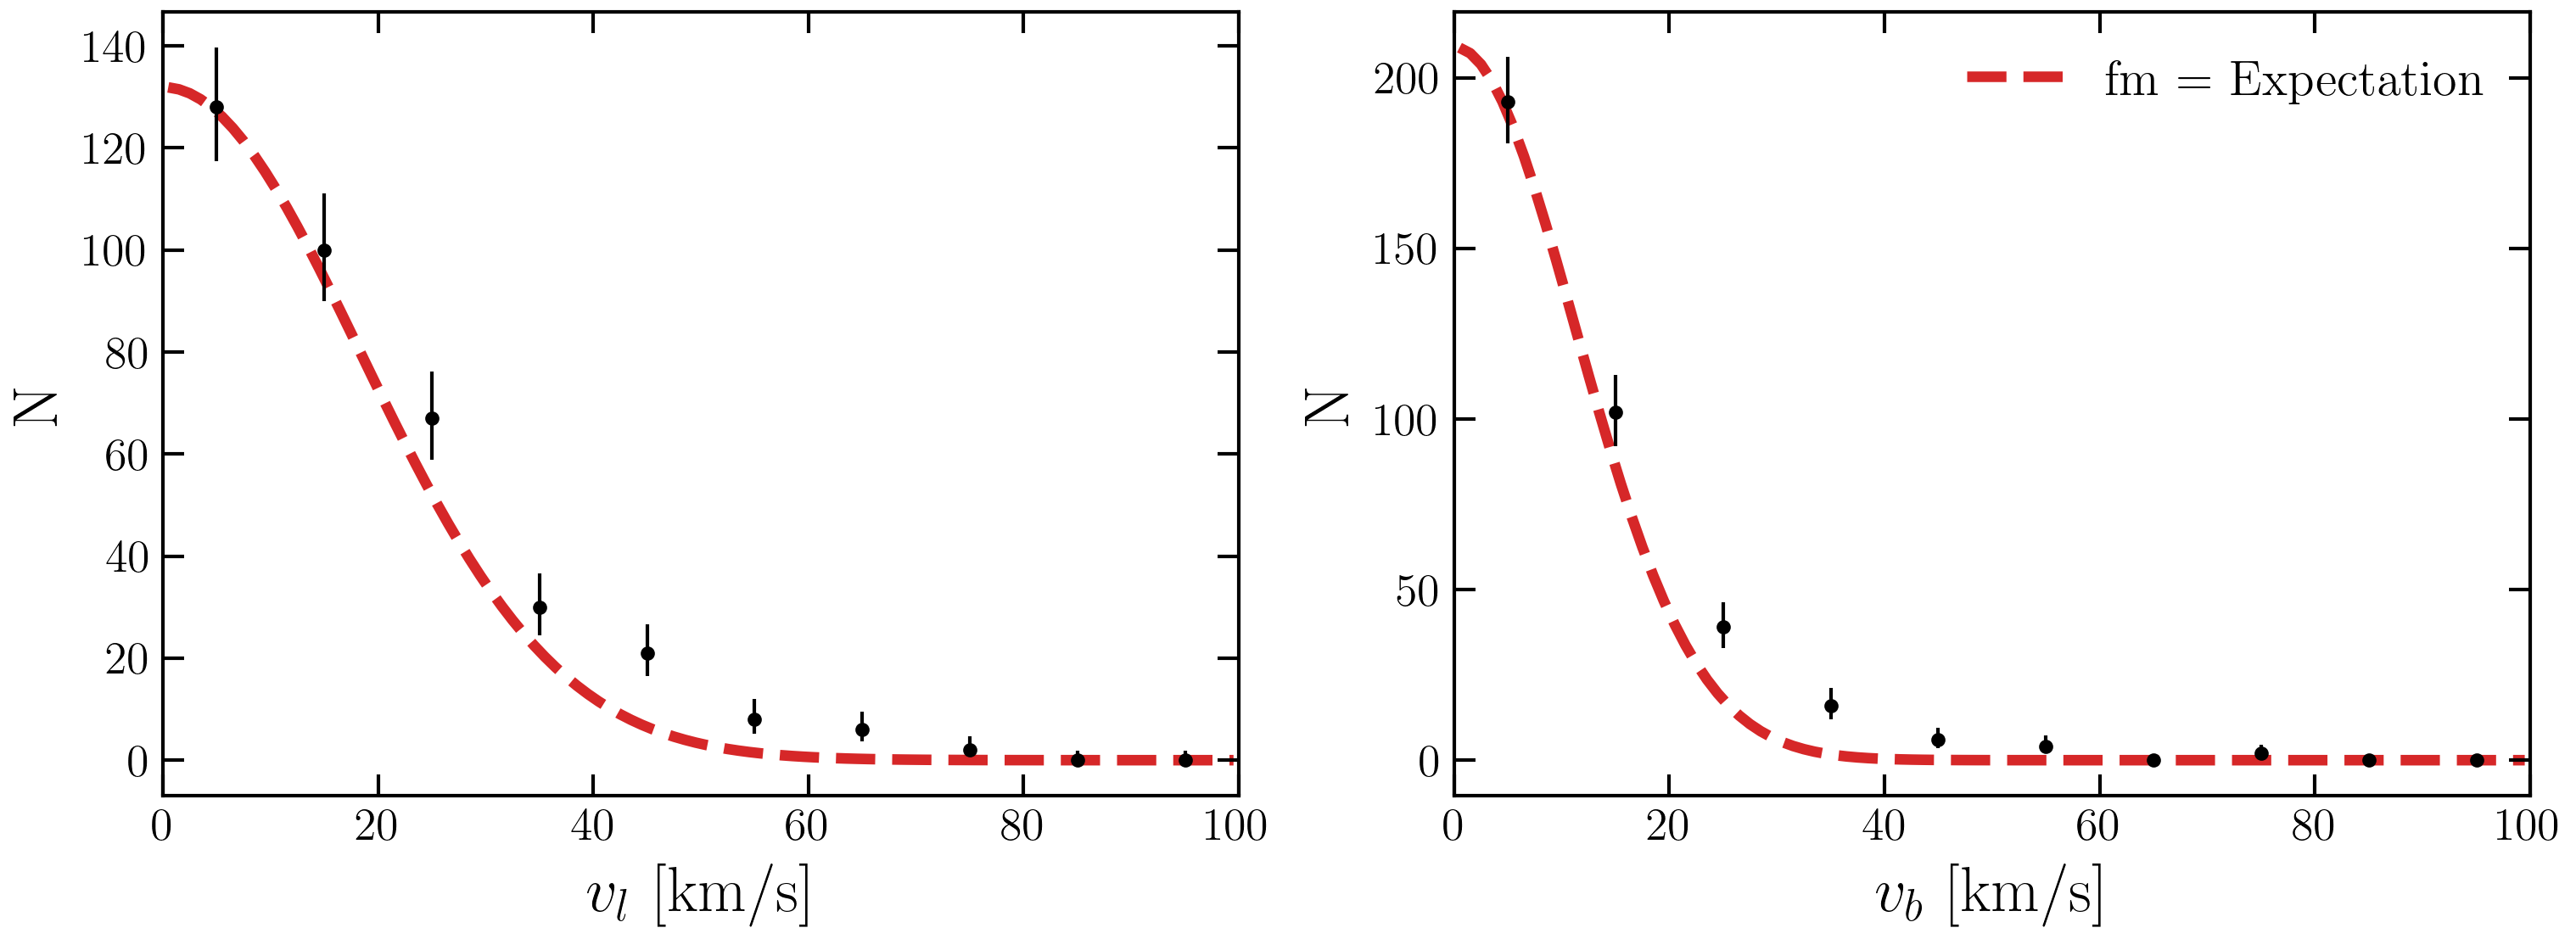
\includegraphics[width=\columnwidth]{vel_dist.png}
%     \caption{The observed velocity dispersion in $v_l$ and $v_b$ for the WD+MS sample described in Section~\ref{sec:AVR} (black points). The expected velocity dispersion given the ages of the white dwarfs in the systems is shown as a dashed red line. Errors are determined through Poisson statistics taken from \cite{1986ApJ...303..336G}.}
%     \label{fig:vel_dispersion}
% \end{figure}

To determine what distribution of ages is needed to reproduce the observed velocity distribution, we calculate the expected velocity dispersion ($\sigma_i$) for a population of stars at constant ages between 0.25 and 10 Gyr with steps of 0.25~Gyr. We fit the observed velocity distributions in $v_l$ and $v_b$ with the following weighted sum;
\begin{equation}
    N_{\mathrm{expected}}(v) = A\sum^{40}_{i=1} w_i \exp{(-v/2\sigma_i)^2}
\end{equation}
where $A$ is a normalization factor, $w_i$ is a weighting factor, and $\sigma_i$ is the expected velocity dispersion of the $i^{\mathrm{th}}$ age. We find that a population of very old ($>7$~Gyr) stars in the sample could explain the discrepancy between the expected and observed velocity distributions at the level of around 30\% (see Figure~\ref{fig:vel_fit}). It is important to note that the fit we have done is highly degenerate, with 40 separate weighting factors being fit. We run the fit 100 times with random starting positions and find the simulated age distribution does not change significantly over the 100 runs.

% \begin{figure}
%     \centering
%     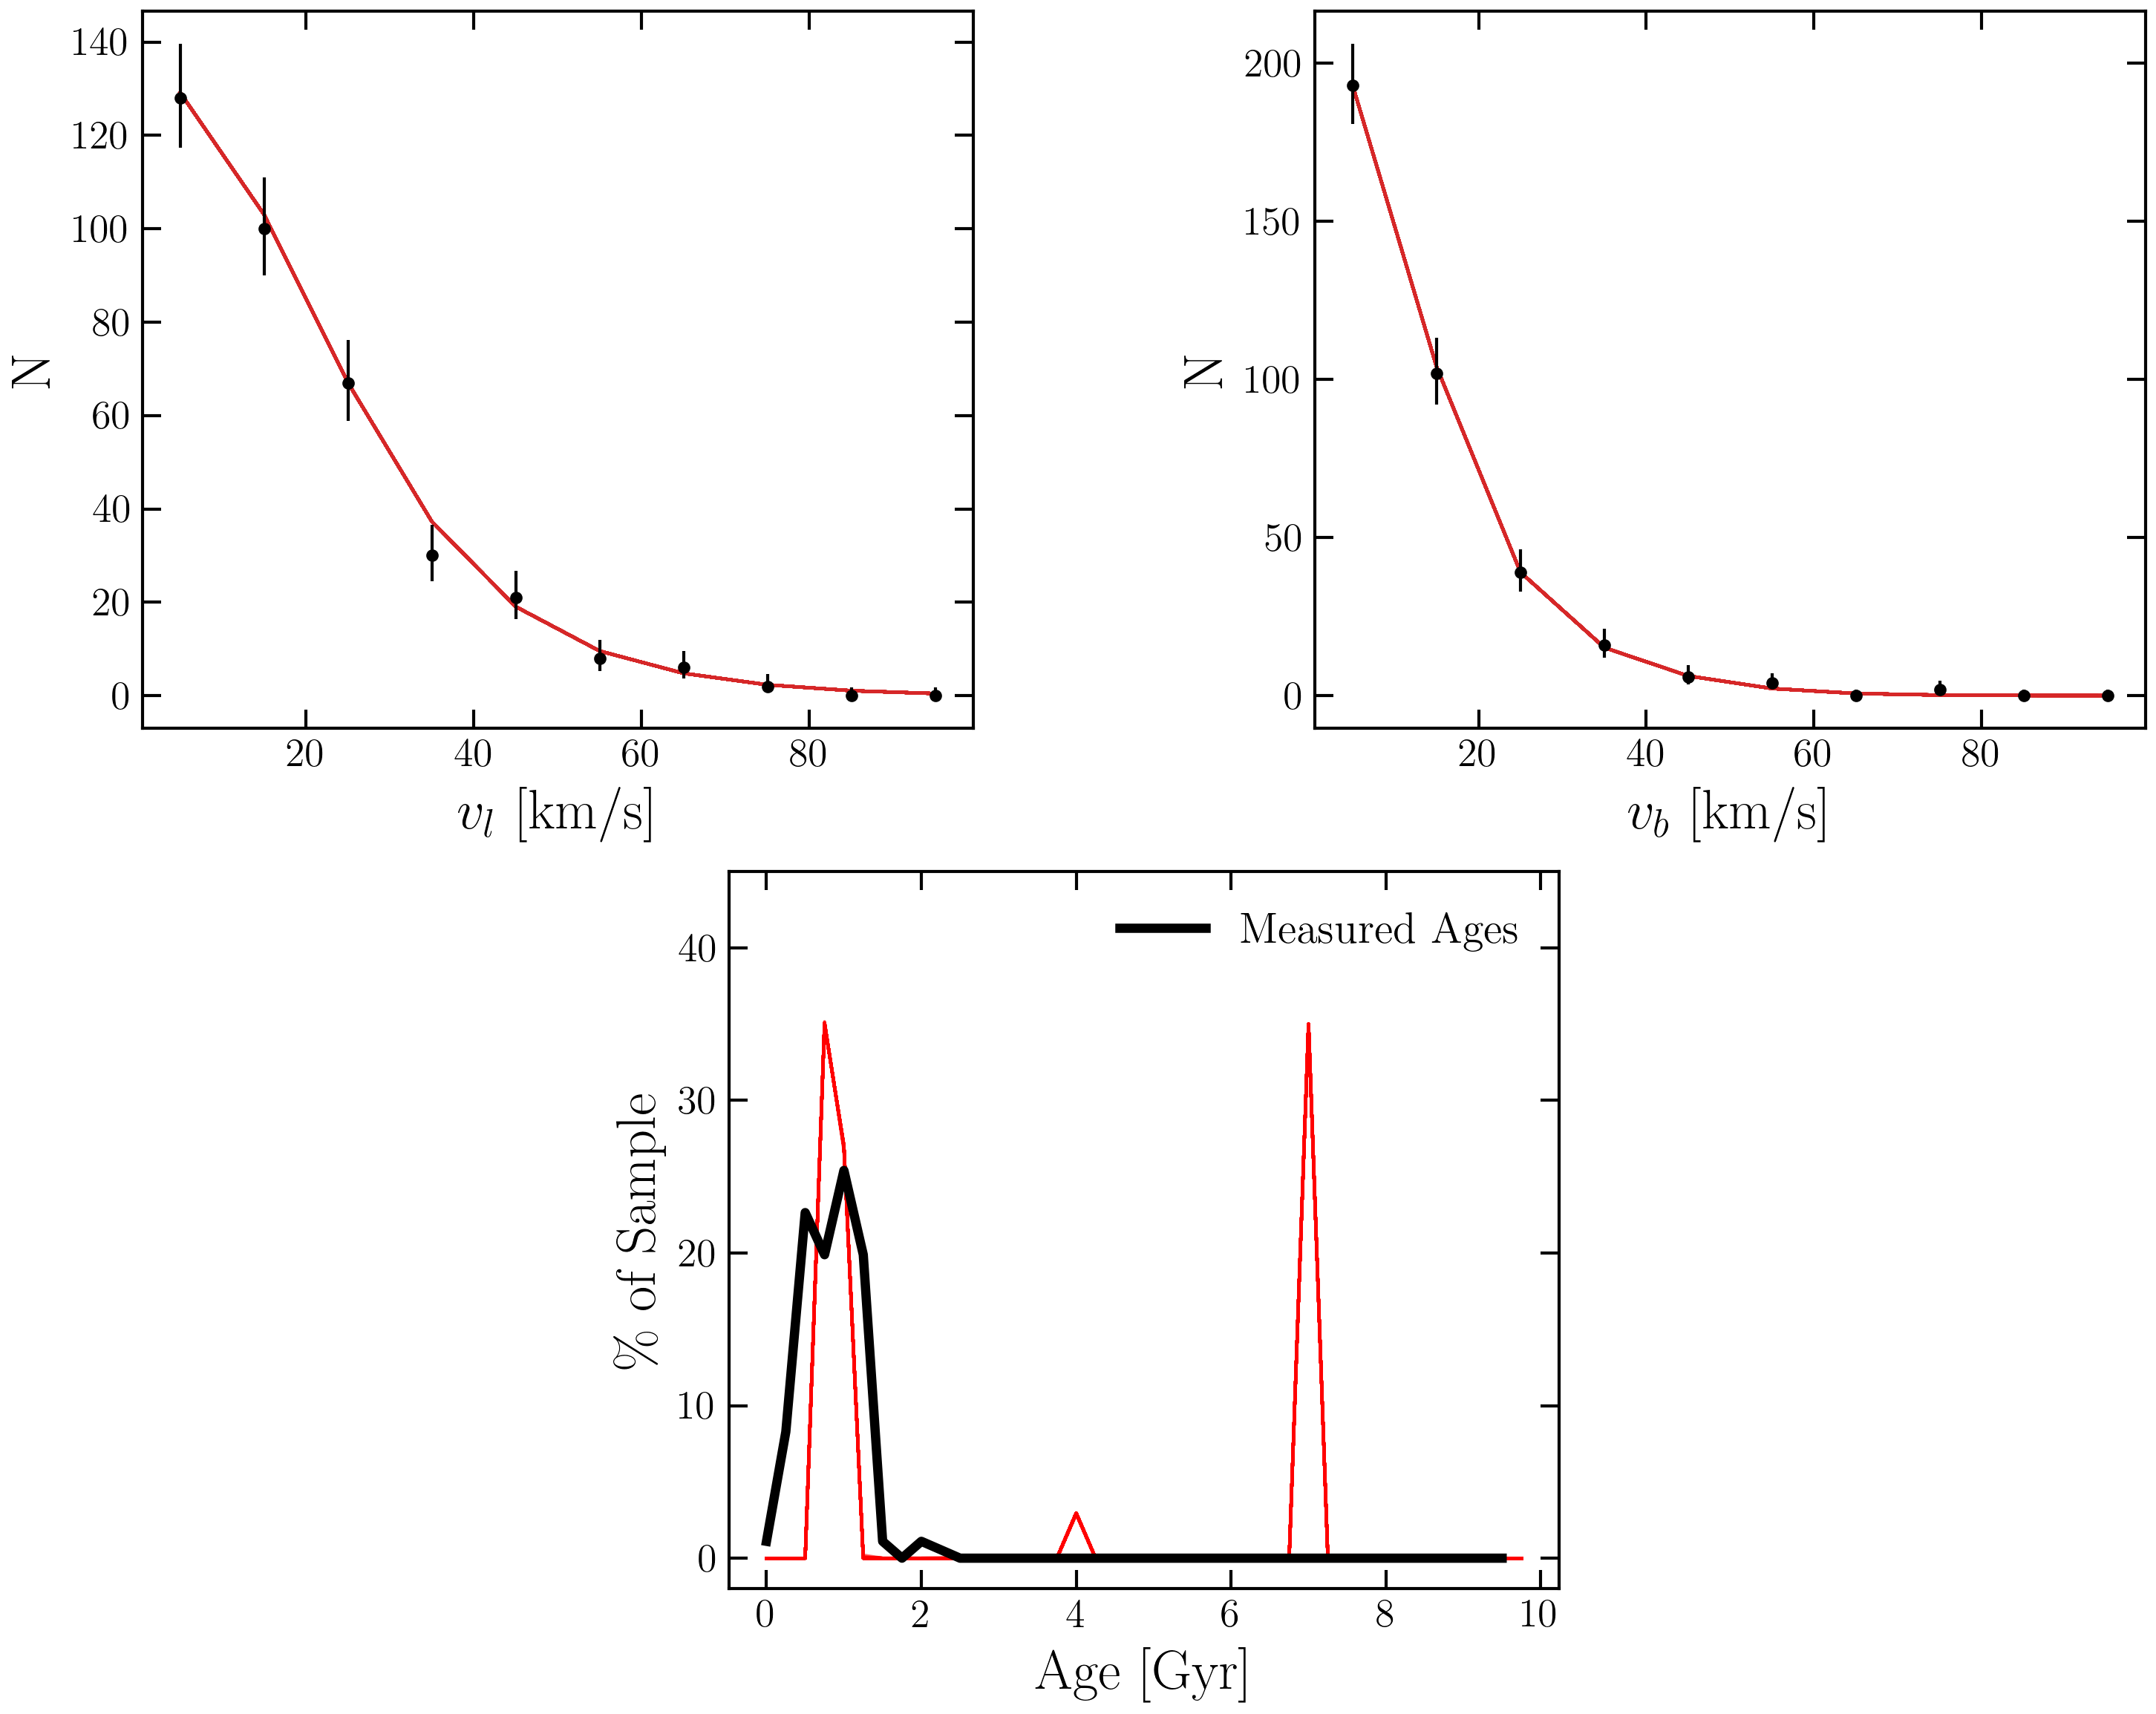
\includegraphics[width=\columnwidth]{vel_fit.png}
%     \caption{A fit to the velocity distributions in $v_l$ and $v_b$ of the sample of WD+MS binaries described in Section~\ref{sec:AVR}. The black points are the observed velocity distribution with errors determined through Poisson statistics taken from \cite{1986ApJ...303..336G}. The red line shows the best fit velocity distribution described in Section~\ref{sec:AVR}. The bottom panel shows the observed age distribution of the sample in black and the corresponding age distribution to produce the best fitting velocity distribution in red. An older population with a larger velocity dispersion is needed to alleviate the discrepancy between the observed and expected velocity distribution shown in Figure~\ref{fig:vel_dispersion}.}
%     \label{fig:vel_fit}
% \end{figure}

Thus, it is clear that a much older population is necessary to reproduce the observed velocities in the sample. There are three possible mechanisms for why the white dwarf ages appear underestimated by such a large factor: (1) the models applied to some of the white dwarfs do not accurately represent their true atmospheric composition, (2) there is a high merger fraction in the sample, or (3) some of the wide binary systems are in fact triples where one of the components has a close binary companion.

In the process of determining the spectral type of each white dwarf, we have used spectral types determined through Gaia XP spectra for 141 white dwarfs in the final sample. These spectral types could be incorrect, especially for non-DA determinations \citep{2024ANA...682A...5V}, but in Chapter~\ref{sec:chap3}, we found the number of incorrect determinations was of order a few percent which is not a large enough fraction to account for the discrepancy. We could also be applying the incorrect models to a subset of the DCs in our sample. The process used for determining which models to use (see Section~\ref{sec:age_determ_WDMS}) is determined through the measured effective temperature of the white dwarf. This approach could be applying the wrong models since there is no way to know the exact atmospheric composition of DC white dwarfs. Assuming the incorrect atmospheric model can induce a systematic mass shift on the order of 15\% \citep{2012ApJS..199...29G}. This in turn could underestimate the progenitor lifetime causing these white dwarfs to appear younger. For a $0.7$\msun\ white dwarf, the progenitor lifetime goes from $\sim0.5$~Gyr to $\sim6$~Gyr for the $0.6$\msun\ white dwarf. This effect is diminished for the higher mass white dwarfs where shifts in the white dwarf mass result in progenitor lifetime changes $<1$~Gyr. Again, this is unable to explain the full discrepancy considering only 6\% of the sample are DC or DZ white dwarfs.

The white dwarf ages could be suspect due to the presence of mergers. As discussed in Chapters~\ref{sec:chap2} and \ref{sec:chap3}, mergers are expected to be present in the sample at the $\sim20\%$ level. These mergers preferentially cause the white dwarf ages to be underestimated. This results in high total age errors especially for double white dwarf mergers \citep[e.g.,][]{2014MNRAS.441..354T, 2020A&A...636A..31T}. \cite{2020ApJ...891..160C} were able to show that for high-mass white dwarfs, a merger fraction of 20\% was able to reproduce the observed dispersion of velocities in their sample. 

It is outside the scope of this dissertation to appropriately model the delay time distribution to determine the merger fraction needed to reproduce the observed velocities in the sample, but Figure~\ref{fig:avr_mergers} shows a simple but imperfect approach to determining the approximate merger fraction. The expected velocity distributions in Figure~\ref{fig:avr_mergers} are determined through applying random age corrections between 0 and 5~Gyr to a percentage of the white dwarf ages corresponding to the merger fraction. Then, just as described above for the expected distribution in Figure~\ref{fig:vel_dispersion}, we take an average of the expected velocity dispersions for each white dwarf given the new updated ages. This demonstrates that mergers with a delay time distribution between 0 and 5~Gyr can reproduce the observed velocities.

% \begin{figure}
%     \centering
%     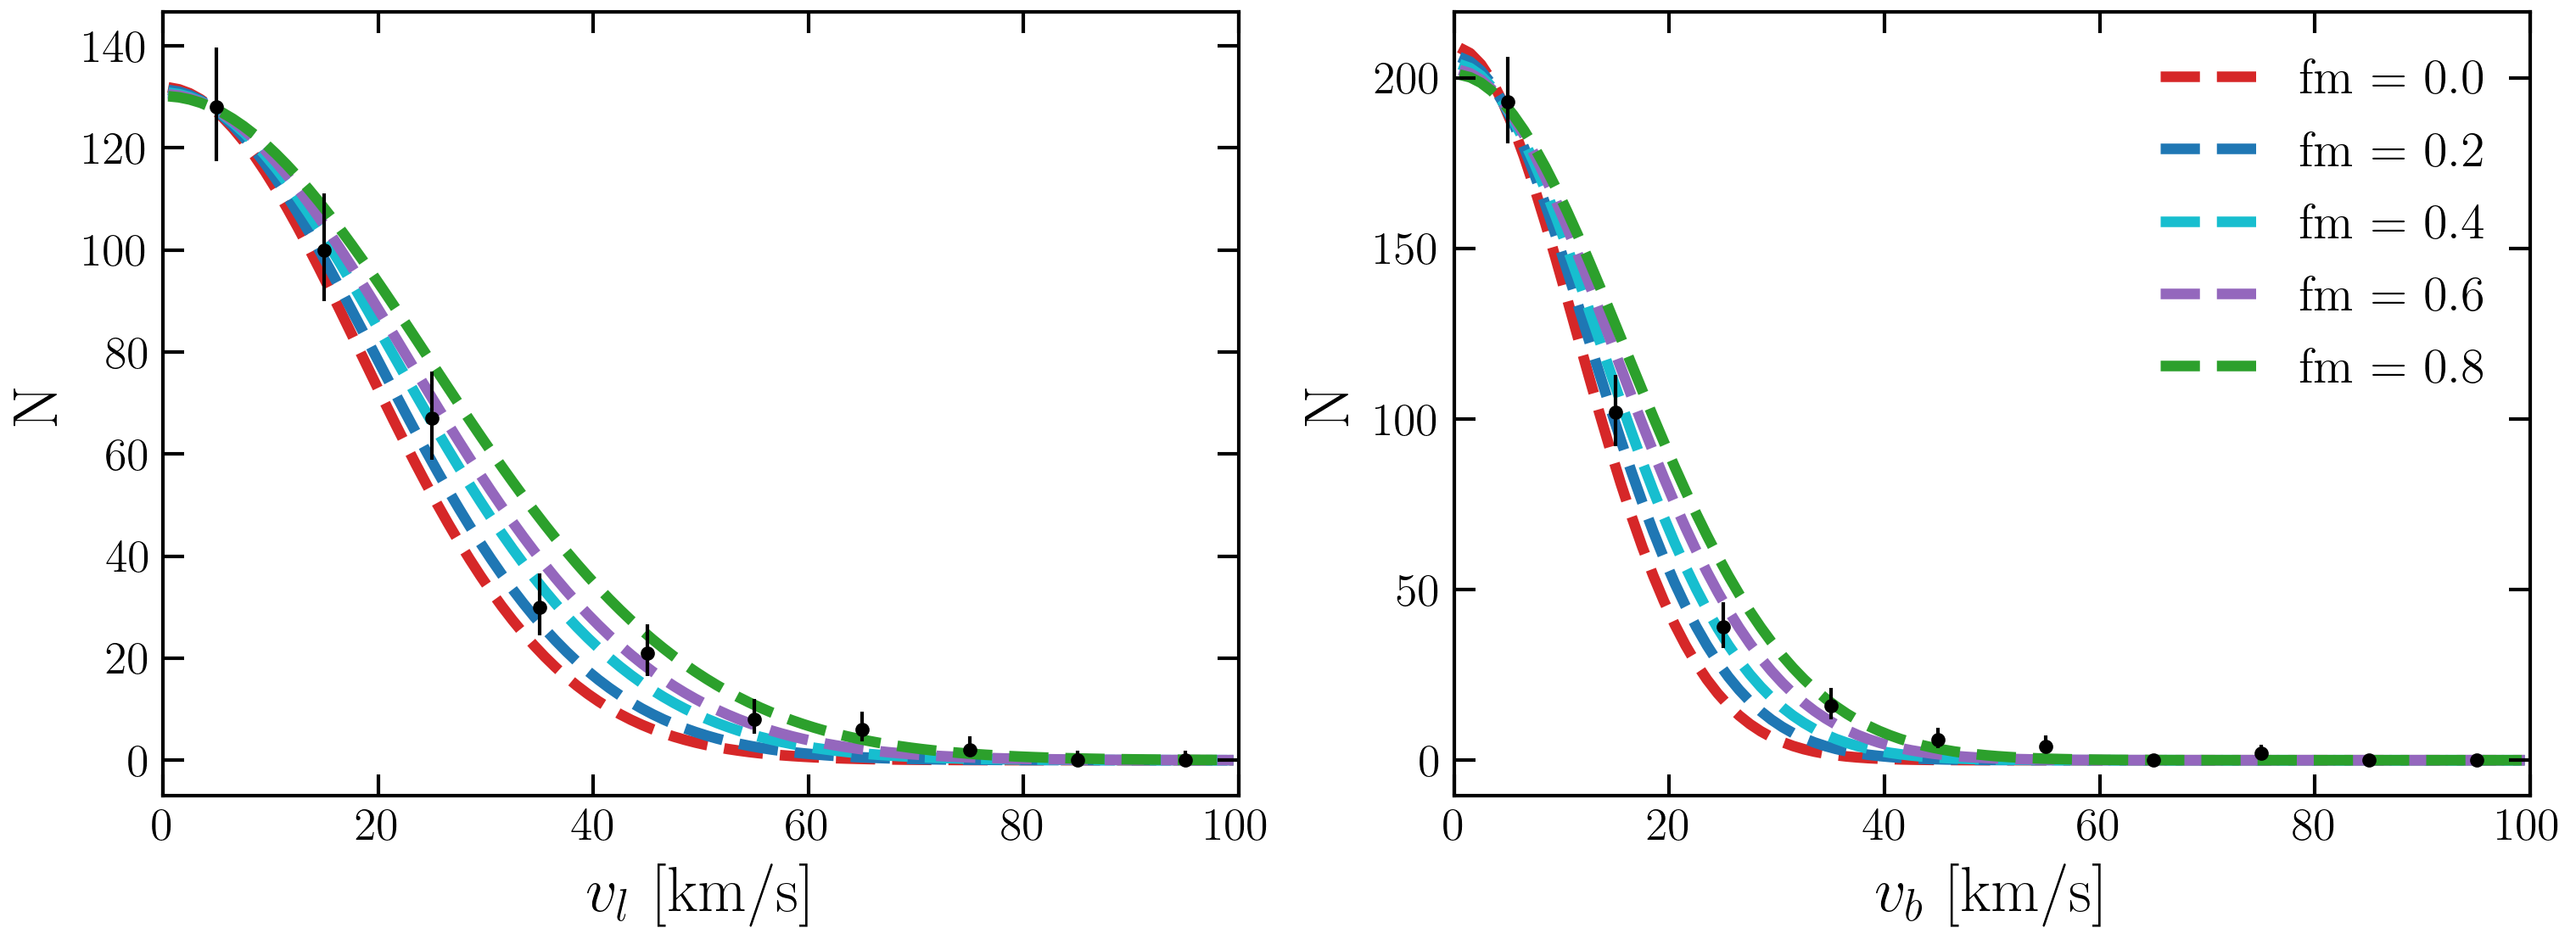
\includegraphics[width=\columnwidth]{vel_dist_mergers.png}
%     \caption{The distribution of velocities in $v_l$ and $v_b$ (black points). Error bars are determined through Poisson statistics taken from \cite{1986ApJ...303..336G}. The expected velocity distributions given a merger fraction are shown as dashed lines.}
%     \label{fig:avr_mergers}
% \end{figure}

Finally, we consider whether a close binary companion to one of the components could be causing issues. The white dwarf could have a close binary companion which is throwing off the SED fit, resulting in incorrect ages. In addition, either the white dwarf or the main-sequence star could have a close binary companion imparting a non-negligible orbital velocity. For the smallest separations in the sample (a few hundred au), the expected circular velocity of the orbit is on the order of a couple km/s. This is not able to explain the observed extra dispersion in the velocities, but if there exist triples in the sample where there is a close binary companion, then the expected orbital velocities begin to approach the level of the observed velocity dispersion with tens of km/s for a separation on the order of one~au.  

It is unclear which of these effects is the largest contributor to the increased velocity dispersion and it is likely that all of these effects are present at some level in the sample.
